\documentclass[10pt,a4paper]{article}
\usepackage[T1]{fontenc}
\usepackage{newtxtext,newtxmath}
\usepackage[margin=2.4cm]{geometry}
\usepackage{graphicx,booktabs,amsmath,caption,subcaption,float,microtype,siunitx,array}
\usepackage[hidelinks]{hyperref}
\captionsetup{font=small,labelfont=bf,skip=4pt}
\emergencystretch=3em\setlength{\parindent}{1.2em}\setlength{\parskip}{0pt}
\renewcommand{\arraystretch}{1.12}
\sisetup{round-mode=none}
\title{\vspace{-1.2cm}\textbf{Smoke-Test Evaluation of CoAtNet-0 on a Curated Brain-MRI Benchmark:\\ Stratified Five-Fold Development with a Reserved External Test Set}}
\author{DERMS-R benchmark pipeline --- run \texttt{smoke-msoud-coatnet0}}
\date{26 November 2026 (run completed 25 November 2026, UTC)}
\begin{document}
\maketitle
\begin{abstract}
\noindent We report a deliberately short ("smoke") training run that exercises the full DERMS-R benchmark pipeline for the \texttt{coatnet\_0} architecture (\texttt{coatnet\_0\_rw\_224.sw\_in1k}, 26.7\,M parameters) on the four-class brain-MRI benchmark \texttt{Msoud\_v2} (4,831 development images). Models were fine-tuned for two epochs under stratified five-fold cross-validation (CV) at five training ratios, $r\in\{0.10,0.25,0.50,0.75,1.00\}$. The DERMS-R criterion selected $r=0.10$, after which the architecture was refitted once and evaluated a single time on a reserved, independently sourced test set (BRISC2025, $n=952$). Cross-validated accuracy rose monotonically from 0.840 ($r=0.10$) to 0.976 ($r=1.00$), but the locked model reached only 0.606 accuracy (95\% Wilson CI 0.575--0.637) on the external test set, with macro-F1 of 0.565 and one-vs-rest macro AUC of 0.888. Errors concentrated in glioma$\rightarrow$meningioma and no-tumor$\rightarrow$pituitary confusions. Grad-CAM maps for one randomly drawn test image per class were generated and logged to MLflow; in three of four examples the attribution fell largely on the skull, the image margin or non-brain tissue, and in the glioma example the visible lesion received little weight. Because the run is intentionally under-trained and the CV folds were not grouped by near-duplicate or patient, these figures verify the pipeline and characterise the cross-source gap; they should not be read as the attainable performance of the architecture.
\end{abstract}

\section{Introduction}
The purpose of this run was operational: to confirm that the newly registered architecture \texttt{coatnet\_0} and the newly registered datasets train, cross-validate, lock and test correctly end-to-end on the RTX~5000 (Ada) host, before committing GPU time to a full benchmark. The run follows the DERMS-R protocol, in which an architecture is trained at several fractions of the development data, scored by a composite criterion that rewards accuracy, data efficiency, parameter efficiency and fold-to-fold stability, refitted at the selected ratio, and evaluated exactly once on a held-out test partition that is never used for model or ratio selection.

\section{Materials and Methods}
\subsection{Data}
The development partition is a curated subset of the Msoud brain-tumor MRI collection (Kaggle, version~2; \texttt{Msoud\_v2\_development\_curated\_provisional\_v1}) and contains 4,831 images in four classes (glioma 1,313, meningioma 1,106, no tumor 1,266, pituitary 1,146). The test partition is a curated subset of the BRISC2025 collection (Kaggle, version~6; \texttt{BRISC2025\_v6\_test\_curated\_provisional\_v1}) with 952 images (glioma 244, meningioma 294, no tumor 139, pituitary 275). The two packages share no image by SHA-256 and use an identical class-to-index mapping. Both packages are marked by their authors as \emph{provisional automated selections}: manual curation is incomplete, near-duplicate grouping within Msoud has not been finalised, and patient- or source-level independence has not been established. The test class distribution differs from development (no-tumor 14.6\% vs.\ 26.2\%), and the two sources originate from different repositories, so the test measures cross-source transfer in addition to generalisation.

\subsection{Model and training}
We used \texttt{coatnet\_0\_rw\_224.sw\_in1k} from \texttt{timm} 1.0.29 with ImageNet-1k pretrained weights and a freshly initialised four-way classification head. Images were resized to $224\times224$ and normalised with ImageNet statistics. Training used AdamW (weight decay 0.01), a cosine-annealed learning rate starting at $10^{-4}$ (annealed over the two epochs; $5\times10^{-5}$ in the second epoch), batch size 32, full-precision (float32) arithmetic, and the repository's default augmentation policy (flip, rotation up to $20^{\circ}$, HSV/LAB colour jitter, brightness/contrast, Gaussian noise and blur). Each fit ran for 2 epochs; with \texttt{--epoch-selection last} the final epoch is always evaluated, so no checkpoint is chosen using validation data.

\begin{table}[H]\centering\small
\caption{Run configuration (from \texttt{config.json}).}\label{tab:setup}
\begin{tabular}{ll@{\hspace{2.2em}}ll}
\toprule
Architecture & \texttt{coatnet\_0\_rw\_224.sw\_in1k} & Epochs per fit & 2 \\
Parameters & 26,669,638 & Batch size & 32 \\
CV strategy & \texttt{StratifiedKFold}, 5 folds & Learning rate / weight decay & $10^{-4}$ / 0.01 \\
Training ratios & 0.10, 0.25, 0.50, 0.75, 1.00 & Epoch selection & last epoch \\
Seed & 42 & Pretrained & yes (ImageNet-1k) \\
GPU & NVIDIA RTX 5000 Ada Generation & Software & PyTorch 2.4.1, timm 1.0.29 \\
\bottomrule
\end{tabular}
\end{table}

\subsection{Protocol and scoring}
For each ratio $r$, a stratified subset of the development partition was drawn and divided into five folds; each fold served once as validation data. For every $r$ the five validation accuracies yield a mean $\bar A$ and unbiased standard deviation $s$. The DERMS-R score is the product of four components,
\begin{equation}
\text{DERMS-R}(r)=\underbrace{\bar A^{\alpha}}_{\text{performance}}\cdot\underbrace{r^{-\gamma}}_{\text{data eff.}}\cdot\underbrace{(P/P_0)^{-\beta}}_{\text{complexity eff.}}\cdot\underbrace{(1+s/\sigma_0)^{-\delta}}_{\text{stability}},
\end{equation}
with $\alpha=2$, $\gamma=\beta=\delta=0.5$, $P_0=10^{6}$ parameters and $\sigma_0=10^{-3}$ (canonical values), where $P$ is the number of trainable parameters. The ratio with the highest DERMS-R was locked; the model was then refitted once on the corresponding stratified subset (481 images, realised ratio 0.0996) for the median best epoch of its folds (2) and evaluated once on the BRISC2025 test partition. Test metrics were computed from the stored predictions and probabilities: accuracy with a 95\% Wilson interval, per-class precision, recall and F1, macro-F1, Matthews correlation coefficient (MCC), and one-vs-rest ROC AUC. The test set was not used for any selection.

\subsection{Grad-CAM}
To inspect which image regions drive the locked model's decisions we computed Grad-CAM maps\footnote{Selvaraju et al., ``Grad-CAM: Visual explanations from deep networks via gradient-based localization'', ICCV 2017.} on the test set for one image per class. Images were drawn uniformly at random within each class with a fixed seed (42) so that the examples are not hand-picked. The target layer is the output of the last CoAtNet stage ($7\times7$ spatial resolution); channel weights are the spatially averaged gradients of the class logit, the weighted sum is rectified, bilinearly upsampled to $224\times224$ and min--max normalised per image. Maps are shown for the predicted class and, for misclassified images, also for the true class. Predictions recomputed in this analysis were asserted to equal those stored by the test run, and the checkpoint was verified against the SHA-256 recorded in the lock file. Grad-CAM is a qualitative aid: its localisation is coarse, it was not validated here against lesion annotations, and it does not establish that a region is causally used by the network.

\section{Results}
\subsection{Cross-validation}
Cross-validated accuracy increased monotonically with the training ratio, from 0.840 at $r=0.10$ to 0.976 at $r=1.00$, and the fold-to-fold standard deviation shrank from 0.022 to 0.007 (Table~\ref{tab:cv}, Fig.~\ref{fig:cv}a). The parameter-efficiency component is constant across ratios (0.194), so DERMS-R is decided by the trade-off between the performance, data-efficiency and stability terms (Table~\ref{tab:comp}). The data-efficiency term $r^{-1/2}$ penalises large ratios more strongly than the squared accuracy rewards them, so the score decreases monotonically from 0.0894 at $r=0.10$ to 0.0661 at $r=1.00$ (Fig.~\ref{fig:cv}b) and the smallest ratio is locked. This is a property of the metric under these hyper-parameters, not evidence that 10\% of the data suffices.

\begin{table}[H]\centering\small
\caption{Five-fold cross-validation results for \texttt{coatnet\_0} on \texttt{Msoud\_v2}. $n_\text{train}$ is the mean training-fold size; metrics are fold means (macro-averaged where applicable). $^{\dagger}$Locked ratio.}\label{tab:cv}
\begin{tabular}{ccccccc}
\toprule
$r$ & $n_\text{train}$ & Accuracy (mean $\pm$ s.d.) & Macro-F1 & MCC & Macro AUC & DERMS-R \\
\midrule
0.10 & 385 & 0.840 $\pm$ 0.022 & 0.825 & 0.796 & 0.976 & 0.0894 $^{\dagger}$ \\
0.25 & 965 & 0.931 $\pm$ 0.014 & 0.928 & 0.909 & 0.992 & 0.0856 \\
0.50 & 1931 & 0.953 $\pm$ 0.011 & 0.952 & 0.938 & 0.997 & 0.0721 \\
0.75 & 2896 & 0.961 $\pm$ 0.008 & 0.960 & 0.948 & 0.998 & 0.0693 \\
1.00 & 3865 & 0.976 $\pm$ 0.007 & 0.976 & 0.968 & 0.998 & 0.0661 \\
\bottomrule
\end{tabular}
\end{table}

\begin{table}[H]\centering\small
\caption{DERMS-R components by training ratio (parameter count $P=26,669,638$).}\label{tab:comp}
\begin{tabular}{cccccc}
\toprule
$r$ & Performance $\bar A^{2}$ & Data eff. $r^{-1/2}$ & Complexity eff. & Stability & DERMS-R \\
\midrule
0.10 & 0.706 & 3.162 & 0.194 & 0.207 & 0.0894 \\
0.25 & 0.866 & 2.000 & 0.194 & 0.255 & 0.0856 \\
0.50 & 0.909 & 1.414 & 0.194 & 0.290 & 0.0721 \\
0.75 & 0.924 & 1.155 & 0.194 & 0.336 & 0.0693 \\
1.00 & 0.953 & 1.000 & 0.194 & 0.358 & 0.0661 \\
\bottomrule
\end{tabular}
\end{table}

\begin{figure}[H]\centering
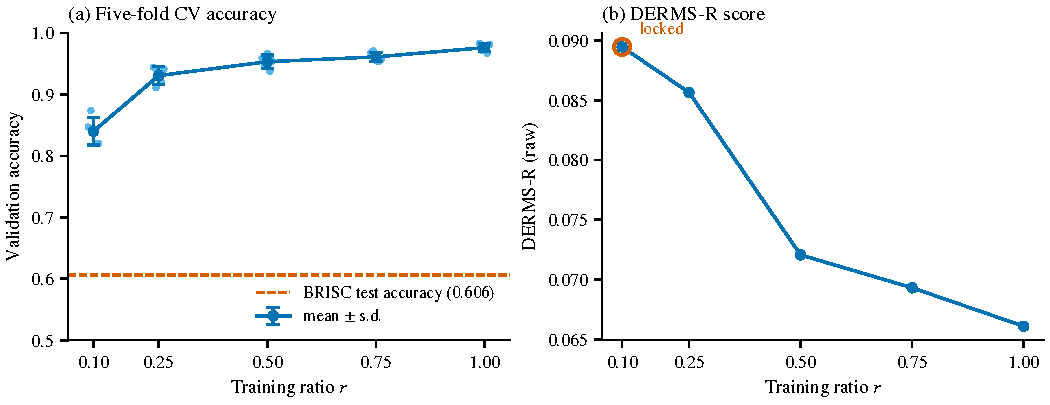
\includegraphics[width=\linewidth]{figures/fig1_cv_ratio.pdf}
\caption{(a) Validation accuracy of the five folds (light points) with mean $\pm$ s.d. (dark) against the training ratio; the dashed line marks the external test accuracy of the locked model. (b) DERMS-R score against the training ratio; the circle marks the locked ratio.}\label{fig:cv}
\end{figure}

\subsection{External test}
The locked model (trained on 481 development images for two epochs) classified 577 of 952 test images correctly: accuracy 0.606 (95\% CI 0.575--0.637), balanced accuracy 0.571, macro-F1 0.565, MCC 0.477 and macro AUC 0.888. The majority-class rate is 0.309, so the model is clearly above chance but 0.234 below its own CV accuracy at the locked ratio and 0.370 below the CV accuracy at $r=1.00$. Per-class results are in Table~\ref{tab:cls}, the confusion matrix in Table~\ref{tab:cm} and Fig.~\ref{fig:cm}, and ROC curves in Fig.~\ref{fig:roc}a.

\begin{table}[H]\centering\small
\caption{Per-class results of the locked model on the BRISC2025 test set.}\label{tab:cls}
\begin{tabular}{lccccc}
\toprule
Class & Support & Precision & Recall & F1 & ROC AUC \\
\midrule
Glioma & 244 & 1.000 & 0.410 & 0.581 & 0.961 \\
Meningioma & 294 & 0.546 & 0.527 & 0.536 & 0.706 \\
No tumor & 139 & 0.442 & 0.360 & 0.397 & 0.905 \\
Pituitary & 275 & 0.598 & 0.989 & 0.745 & 0.978 \\
\midrule
Macro average & 952 & 0.647 & 0.571 & 0.565 & 0.888 \\
\bottomrule
\end{tabular}
\end{table}

\begin{table}[H]\centering\small
\caption{Test confusion matrix (rows: true class; columns: predicted class).}\label{tab:cm}
\begin{tabular}{lccccr}
\toprule
 & Glioma & Meningioma & No tumor & Pituitary & True total \\
\midrule
Glioma & \textbf{100} & 103 & 0 & 41 & 244 \\
Meningioma & 0 & \textbf{155} & 63 & 76 & 294 \\
No tumor & 0 & 23 & \textbf{50} & 66 & 139 \\
Pituitary & 0 & 3 & 0 & \textbf{272} & 275 \\
\midrule
Predicted total & 100 & 284 & 113 & 455 & 952 \\
\bottomrule
\end{tabular}
\end{table}

\begin{figure}[H]\centering
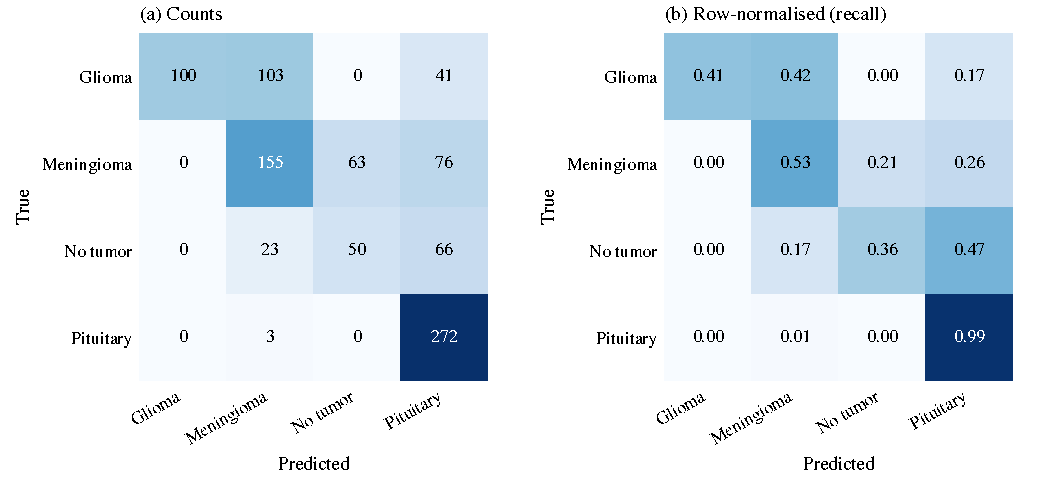
\includegraphics[width=\linewidth]{figures/fig2_test_confusion.pdf}
\caption{Confusion matrix of the locked model on the external test set, as counts (a) and row-normalised recall (b).}\label{fig:cm}
\end{figure}

The errors are systematic rather than diffuse. 42.2\% of glioma images were labelled meningioma and a further 16.8\% pituitary, giving a glioma recall of 0.410. 47.5\% of no-tumor images were predicted as pituitary and 16.5\% as meningioma (recall 0.360), while 21.4\% of meningiomas were predicted as no tumor. Pituitary recall is high (0.989) but precision is only 0.598 because the model predicts pituitary for 455 images against 275 true cases: the classifier is biased toward this class on the new source. Fig.~\ref{fig:rec} contrasts per-class recall in CV with that on the test set; the drop is largest for glioma and no tumor, and it is already visible against the equally under-trained CV models at $r=0.10$. The one-vs-rest AUCs (Fig.~\ref{fig:roc}a) show that the class scores retain ranking information (glioma 0.961, pituitary 0.978) except for meningioma (0.706), whose probabilities are poorly separated from those of the other classes. Confidence is only modestly lower when the model errs: the mean maximum softmax probability is 0.879 for correct and 0.736 for incorrect predictions (Fig.~\ref{fig:roc}b).

\begin{figure}[H]\centering
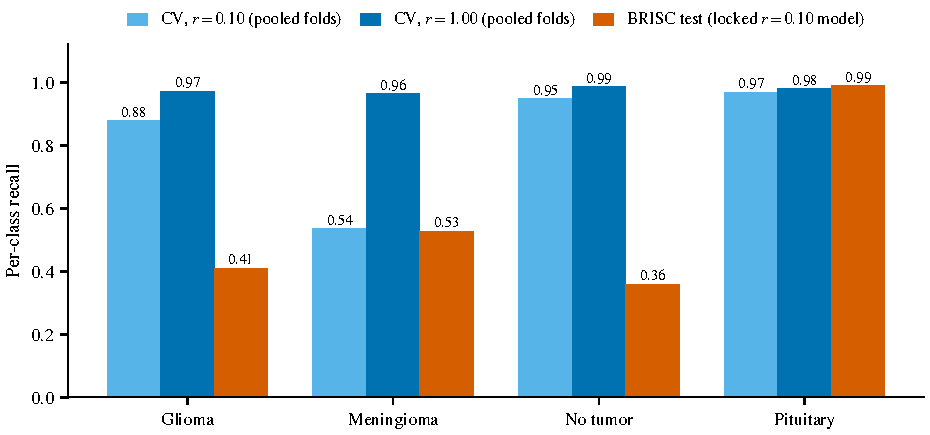
\includegraphics[width=0.86\linewidth]{figures/fig3_recall_cv_vs_test.pdf}
\caption{Per-class recall of pooled cross-validation folds (at the locked ratio $r=0.10$ and at $r=1.00$) versus the external test set.}\label{fig:rec}
\end{figure}

\begin{figure}[H]\centering
\begin{subfigure}[t]{0.49\linewidth}\centering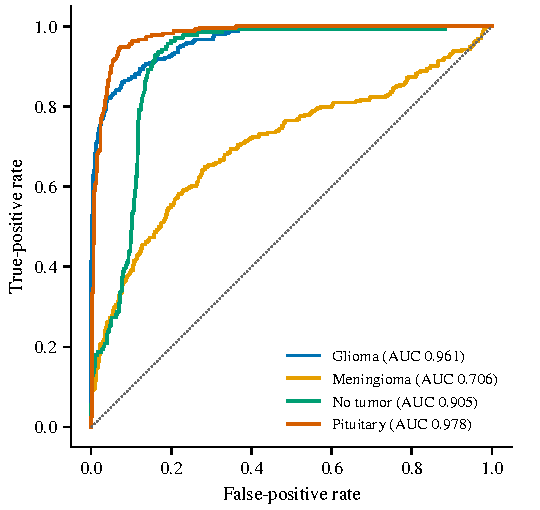
\includegraphics[width=\linewidth]{figures/fig4_test_roc.pdf}\caption{One-vs-rest ROC curves.}\end{subfigure}
\begin{subfigure}[t]{0.49\linewidth}\centering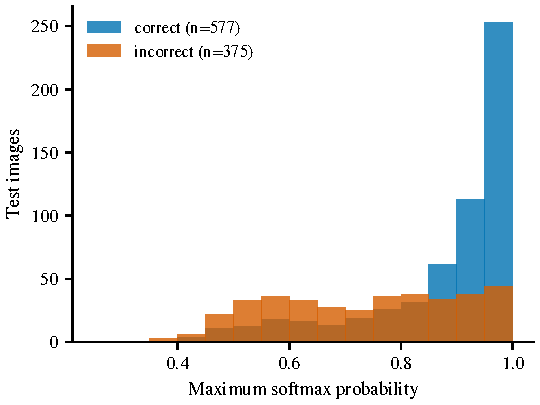
\includegraphics[width=\linewidth]{figures/fig5_confidence.pdf}\caption{Prediction confidence.}\end{subfigure}
\caption{Test-set ROC curves per class and distribution of the maximum softmax probability for correct and incorrect predictions.}\label{fig:roc}
\end{figure}

\subsection{Grad-CAM examples}
Figure~\ref{fig:gc} shows the maps for the four randomly selected test images (Table~\ref{tab:gc}); three were classified correctly and the no-tumor example was predicted as pituitary with probability 0.82. This split is consistent with the overall accuracy but, with $n=4$, carries no statistical weight.

\begin{table}[H]\centering\small
\caption{Randomly selected test images used for Grad-CAM (one per class).}\label{tab:gc}
\begin{tabular}{llccc}
\toprule
True class & Image file & Predicted & Prob. & Correct \\
\midrule
glioma & \texttt{brisc2025\_test\_00022\_gl\_ax\_t1.jpg} & glioma & 0.947 & yes \\
meningioma & \texttt{brisc2025\_test\_00494\_me\_sa\_t1.jpg} & meningioma & 0.844 & yes \\
no tumor & \texttt{brisc2025\_test\_00651\_no\_co\_t1.jpg} & pituitary & 0.819 & no \\
pituitary & \texttt{brisc2025\_test\_00841\_pi\_co\_t1.jpg} & pituitary & 0.973 & yes \\
\bottomrule
\end{tabular}
\end{table}

\begin{figure}[H]\centering
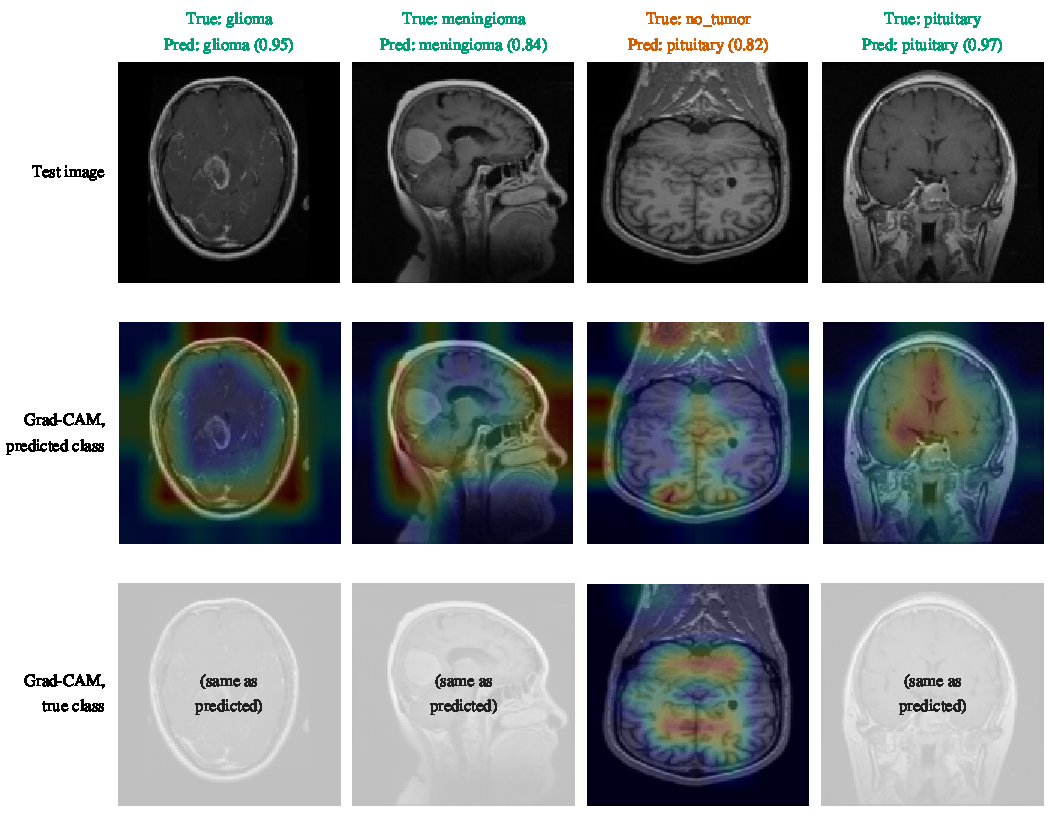
\includegraphics[width=\linewidth]{figures/fig6_gradcam.pdf}
\caption{Grad-CAM for the locked model on one random test image per class: input (top), map for the predicted class (middle) and, where the prediction was wrong, for the true class (bottom). Warmer colours indicate higher attribution; maps are normalised per image.}\label{fig:gc}
\end{figure}

Visual inspection suggests the following, which we state as observations on four images and not as findings. For the correctly classified glioma, attribution is concentrated on the skull margin and the corners of the frame, while the central region containing the visible lesion receives little weight. For the meningioma, the attribution is diffuse and spreads over the skull and facial structures; the bright mass at the left of the image is only weakly highlighted. For the no-tumor image predicted as pituitary, the map of the predicted class is dominated by the upper border of the image (the neck region) and the posterior brain, whereas the map of the true class covers the central cerebellar region. Only for the pituitary example is the attribution concentrated near the midline and suprasellar region, anatomically closer to the expected site. Taken together with the cross-source drop in accuracy, attention to the periphery, to non-brain tissue and to the image frame is compatible with the model using acquisition or framing cues that do not transfer between the two sources; this is a hypothesis for the longer run, to be tested with more images, annotated lesion masks and a faithfulness check such as occlusion or perturbation tests. The map resolution ($7\times7$) and the short two-epoch training may also contribute to the diffuse patterns.

\subsection{Computational profile}
Parameter count and a single-image GPU inference profile were recorded for every fit (Table~\ref{tab:prof}). Latency is the mean over 50 repeats at batch size 1 in float32 and was stable across ratios. The FLOP count is reported as partial by the profiler (several operators, including attention and GELU, are unsupported) and is therefore omitted from the table rather than reported as a lower bound.

\begin{table}[H]\centering\small
\caption{Computational profile of \texttt{coatnet\_0} (RTX~5000 Ada, float32, batch size 1).}\label{tab:prof}
\begin{tabular}{lr}
\toprule
Trainable parameters & 26,669,638 \\
Inference latency, mean over fits (ms) & 3.73 (s.d. 0.01 across fits) \\
Peak CUDA memory during inference (MiB) & 290 \\
Peak CUDA memory during training (GiB) & 5.38 \\
Epoch time, locked refit (s) & 2.6 \\
\bottomrule
\end{tabular}
\end{table}

\section{Discussion and Limitations}
The run met its operational aim: the architecture and the datasets load, train, cross-validate, lock and evaluate end to end, and the reserved test set was opened exactly once. The scientific content is limited by design and by data, and the following caveats apply.
\begin{enumerate}
\item \textbf{Under-training.} Each model saw only two epochs. The locked refit used 481 images. The test accuracy therefore characterises a barely fine-tuned model.
\item \textbf{Ratio selection by DERMS-R.} With the canonical exponents the data-efficiency term dominates and the smallest ratio is always favoured at this accuracy level. The locked model is thus the weakest configuration in CV (Table~\ref{tab:cv}); a production run should inspect the score components rather than rely on the arg-max alone.
\item \textbf{Ungrouped folds.} Folds were stratified by class only. The data package states that near-duplicate grouping within Msoud is not complete and that patient-level independence is unestablished. Near-duplicates or same-patient slices straddling folds would inflate the CV accuracies in Table~\ref{tab:cv} (up to 0.976), and part of the CV--test gap may reflect this leakage rather than domain shift alone. The two effects cannot be separated with the present run.
\item \textbf{Cross-source shift.} The test images come from a different repository, with a different class balance. A fine-tuned network is known to be sensitive to such shifts, and the strongly asymmetric confusions (Fig.~\ref{fig:cm}) are consistent with a source-dependent decision rule. We did not examine image acquisition characteristics, so we make no causal claim.
\item \textbf{Single seed and single test look.} One seed (42) and one evaluation were run; the reported interval reflects test-sample size only, not training variability.
\item \textbf{Qualitative explainability.} Grad-CAM maps cover one image per class, use a coarse $7\times7$ target layer and are unvalidated against lesion annotations; they can generate hypotheses but do not support claims about what the model has learned.
\end{enumerate}
A follow-up run should use grouped cross-validation once near-duplicate groups are available, train for several tens of epochs, report multiple seeds, and consider the per-class recalls and calibration, not accuracy alone, as selection and acceptance criteria.

\section*{Reproducibility}
All numbers and figures in this report were generated programmatically from the artefacts of the run (directory \texttt{smoke-msoud-coatnet0}: \texttt{config.json}, \texttt{Msoud\_v2/summary.csv}, \texttt{fold\_results.csv}, and the \texttt{locked/coatnet\_0/} test files). Configuration hash \texttt{fa1dd30fe368}, split hash \texttt{192740a788a8}, Grad-CAM images and metadata are also logged in MLflow (experiment "derms-r-benchmark - smoke - Msoud\_v2", run \texttt{9bad2a85b27e}). Locked checkpoint SHA-256 \texttt{e2d055be6931}. Software: Python 3.11.9, PyTorch 2.4.1+cu121, timm 1.0.29, CUDA 12.1.
\end{document}
